\documentclass[border=8pt]{standalone}
\usepackage{pgfplots}
\pgfplotsset{compat=1.18}
\begin{document}
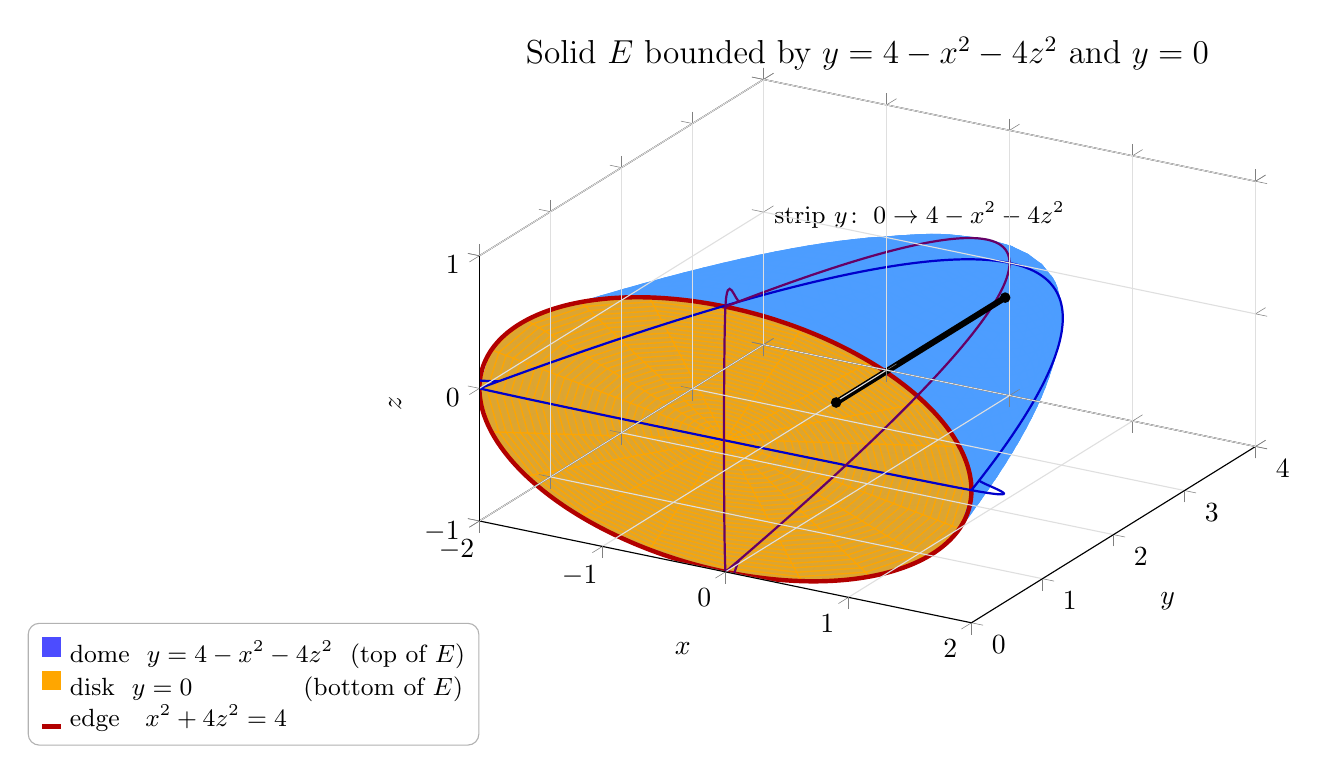
\begin{tikzpicture}
\begin{axis}[
    width = 11.5cm, height = 8.5cm, axis equal image,
    xlabel = $x$, ylabel = $y$, zlabel = $z$,
    xmin = -2, xmax = 2, ymin = 0, ymax = 4, zmin = -1, zmax = 1,
    view = {30}{21},
    grid = major, grid style = {gray!25, line width=.4pt},
    axis on top, samples = 33, samples y = 21,
    domain = 0:1, y domain = 0:360, tick align=outside
]
% 1) paraboloid  y = 4 - x^2 - 4z^2   (parametrised by x = 2r cos t, z = r sin t)
\addplot3[surf, shader=flat, opacity=.95, blue!55!cyan!70!white, draw=none]
    ({2*x*cos(y)}, {4-4*x*x}, {x*sin(y)});
% 2) flat part of the plane y = 0 over the ellipse x^2 + 4z^2 <= 4
\addplot3[surf, shader=flat, opacity=.80, orange!70!yellow, draw=none]
    ({2*x*cos(y)}, {0}, {x*sin(y)});
% 3) common edge: ellipse x^2 + 4z^2 = 4 in the plane y = 0
\addplot3[red!70!black, ultra thick, domain=0:360, samples=181, smooth]
    ({2*cos(x)}, {0}, {sin(x)});
% 4) the two generating parabolas lying on the dome
\addplot3[blue!80!black, thick, domain=-2:2, samples=81, smooth]
    ({x}, {4-x^2}, {0});
\addplot3[violet!80!black, thick, domain=-1:1, samples=81, smooth]
    ({0}, {4-4*x^2}, {x});
% 5) typical strip parallel to the y-axis : y runs from 0 up to 4 - x^2 - 4z^2
\addplot3[black, line width=2.2pt, domain=0:2.38, samples=2]
    ({0.9}, {x}, {0.45});
\addplot3[only marks, mark=*, mark size=1.7pt, black]
    coordinates {(.9,0,.45) (.9,2.38,.45)};
\node[font=\small, text=black] at (axis cs:1.0,1.0,1.55) {strip $y\!:\ 0\to 4-x^2-4z^2$};
\end{axis}
\node[above, font=\large] at (current axis.north)
   {Solid $E$ bounded by $y=4-x^2-4z^2$ and $y=0$};
\node[anchor=north east, align=left, draw=gray!60, fill=white, rounded corners,
      inner sep=5pt, font=\small] at (current axis.south west)
 {{\color{blue!70!white}\rule[2pt]{7pt}{7pt}}\ dome \ $y=4-x^2-4z^2$ \ (top of $E$)\\
  {\color{orange!70!yellow}\rule[2pt]{7pt}{7pt}}\ disk \ $y=0$ \qquad\qquad (bottom of $E$)\\
  {\color{red!70!black}\rule[-1pt]{7pt}{2pt}}\ edge \ \ $x^2+4z^2=4$};
\end{tikzpicture}
\end{document}
